\chapter{Satellite Constellation Management Tools} \label{chapter_tools}
This chapter presents all the scripts designed along this work to achieve the purposes of the thesis.
The first paragraph contains the primary functions needed for the development of the main tools proposed from section \ref{revisit_time_collector_par} to \ref{differential_drag_control_par}.


\section{Orbit Propagators} \label{orbit_propagators_par}
The study of the applications and topics covered by this thesis clearly require an orbital propagator.
The core of all the propagators produced along this work exploit the Cowell's model shown in subsection \ref{orbit_prop_paragraph}.
Both undisturbed and perturbed motion have been analysed.

Orbit propagators must take in input the following data:
\begin{itemize}
    \item \textbf{Initial orbit}. The initial state of the staellite orbit must be defined before propagation.
          All the six orbital elements (see subsection \ref{sat_state_rep_paragraph}) and the epoch are required. 
          The scripts can also work defining the six components of position and velocity vectors.
          Even the TLE can be set as input, which will be appropriately converted into the classical elements representation.  
          The reflectivity coefficient must be added if the problem takes into account the SRP.
    \item \textbf{Time settings}. These input parameters include \textit{time frame} and \textit{time step}.
          The first one simply consists of the total temporal period of propagation requested by the user.
          On the other hand, the time step is strictly related to the output density.
          Lower values imply more detailed results, as well as longer computation times.
          In a nutshell, the outputs will be discretized in as many points as those deriving from the ratio between time frame and time step.
          Small time steps provide narrower plots. 
          Figure \ref{time_step_fig} shows the SMA of a LEO satellite under drag perturbation during one orbit (around 50 minutes). 
          The assigned time step is of 5 minutes (the curve is therefore discretized into 10 points).
          It is important to underline that the accuracy of the integrator used by thesis does not depend on this time step value at all.
    \item \textbf{Perturbations parameters}. Propagators that involve any perturbing acceleration need the parameters which describe that force. 
          For example, the perturbing specific force of atmospheric drag (equation \ref{eq:drag_acc}) requires the air density, which will be given by a specific atmospheric model.
          Even for the acceleration of an eventual thruster it is necessary to specify the force it generates.
    \item \textbf{Spacecraft specifications}. According to the features of the selected propagator, one or more satellite characteristics shall be provided when considering perturbations.
          For instance, in presence of atmospheric drag, $C_D$ and $BC$ (which means cross-sectional area and mass) are needed. 
    \item \textbf{Relative tolerance}. It represents the admitted percent error at any step of the simulation. 
          For instance, a relative tolerance of 0.01 indicates a 1\% allowable error limit relative to each state value at each step.
          This setting controls the accuracy of the solution of the selected integrator \cite{rocha2018numerical} (DOPRI$8_{(5,3)}$ is the method used by the thesis).
\end{itemize}

\begin{figure}[h]
      \centering
      %\textbf{Your title}\par\medskip
      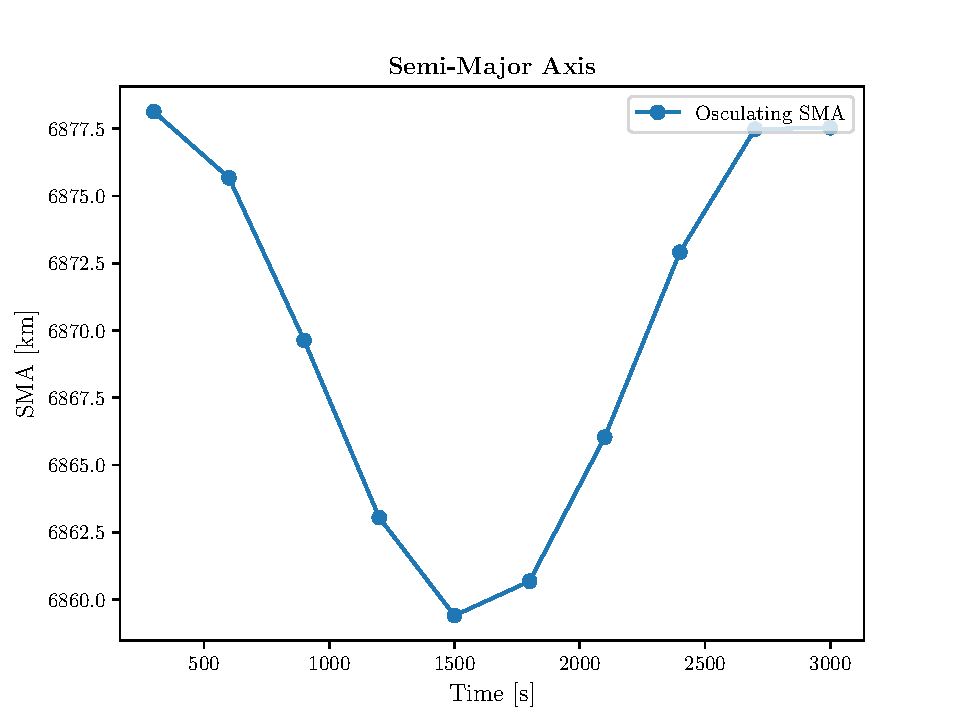
\includegraphics[scale=0.8]{img/time_step.pdf}
      \caption{Osculating SMA of a LEO satellite during one orbit. Propagation time settings: time step = 5 minutes, time frame = 50 minutes.}
      \label{time_step_fig}
  \end{figure}

\subsection{Undisturbed Motion}
The first orbit propagator proposed by this thesis consists of the ideal motion of a spacecraft neglecting all the possible perturbations that might affect it.
Therefore, this kind of propagation is governed by the two-body equation shown in subsection \ref{twobody_par}.

This model is mainly useful for two reasons.
First, it requires computation times definitely shorter than a perturbed propagation, allowing quick results when perturbations are not considered decisive for the purposes of the user.
Secondly, it provides an educational method to better understand the perturbing effects when compared to more realistic propagators.

Figure \ref{kep_low_ecc_fig} shows the orbital elements values of the motion of a satellite in LEO.
\begin{figure}[h]
      \centering
      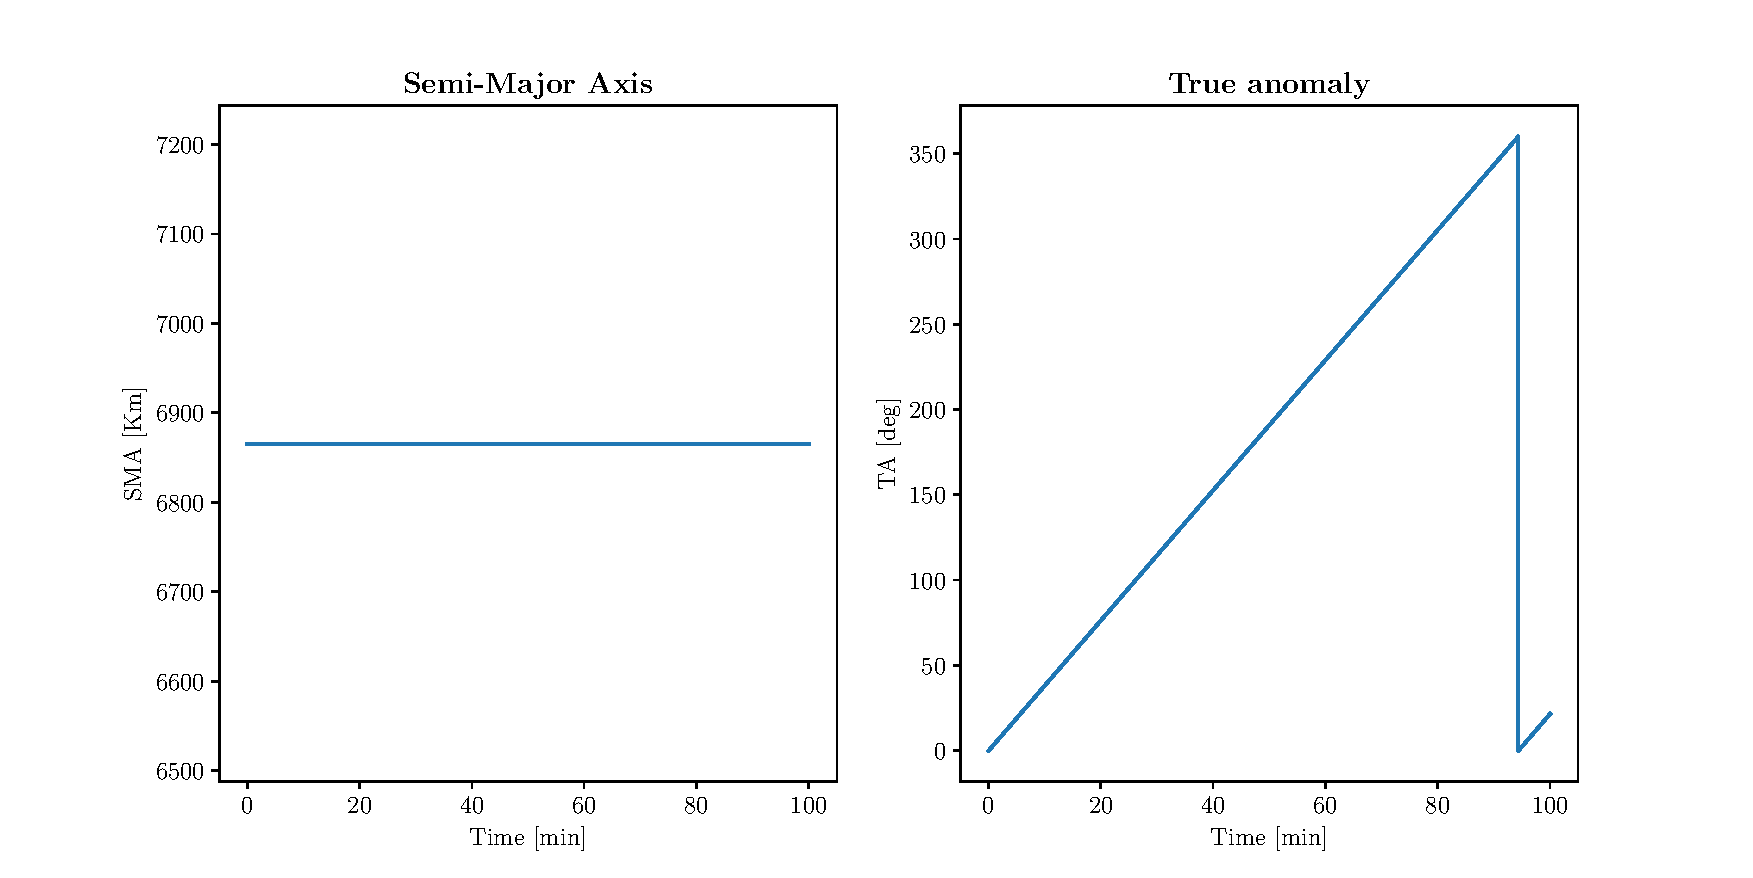
\includegraphics[scale=0.5]{img/keplerian_elements_low_ecc.pdf}
      \caption{SMA and true anomaly variation along around one LEO satellite orbit with eccentricity of 0.001}
      \label{kep_low_ecc_fig}
\end{figure}
Only SMA and true anomaly are reported for matters of layout.
The graph of the other elements is constant like the semi-major axis, because no perturbation affects their behavior.
The true anomaly is the only time-variant parameter, and in this case its curve looks like varying constantly.
The reason of this aspect lies in the eccentricity: this example is characterized by a near-circular orbit, therefore the velocity of the satellite is almost the same along the entire orbit.
Increasing the eccentricity value, like in figure \ref{kep_high_ecc_fig}, the true anomaly changes more rapidly when is in proximity of the perigee and vice-versa.
\begin{figure}[h]
      \centering
      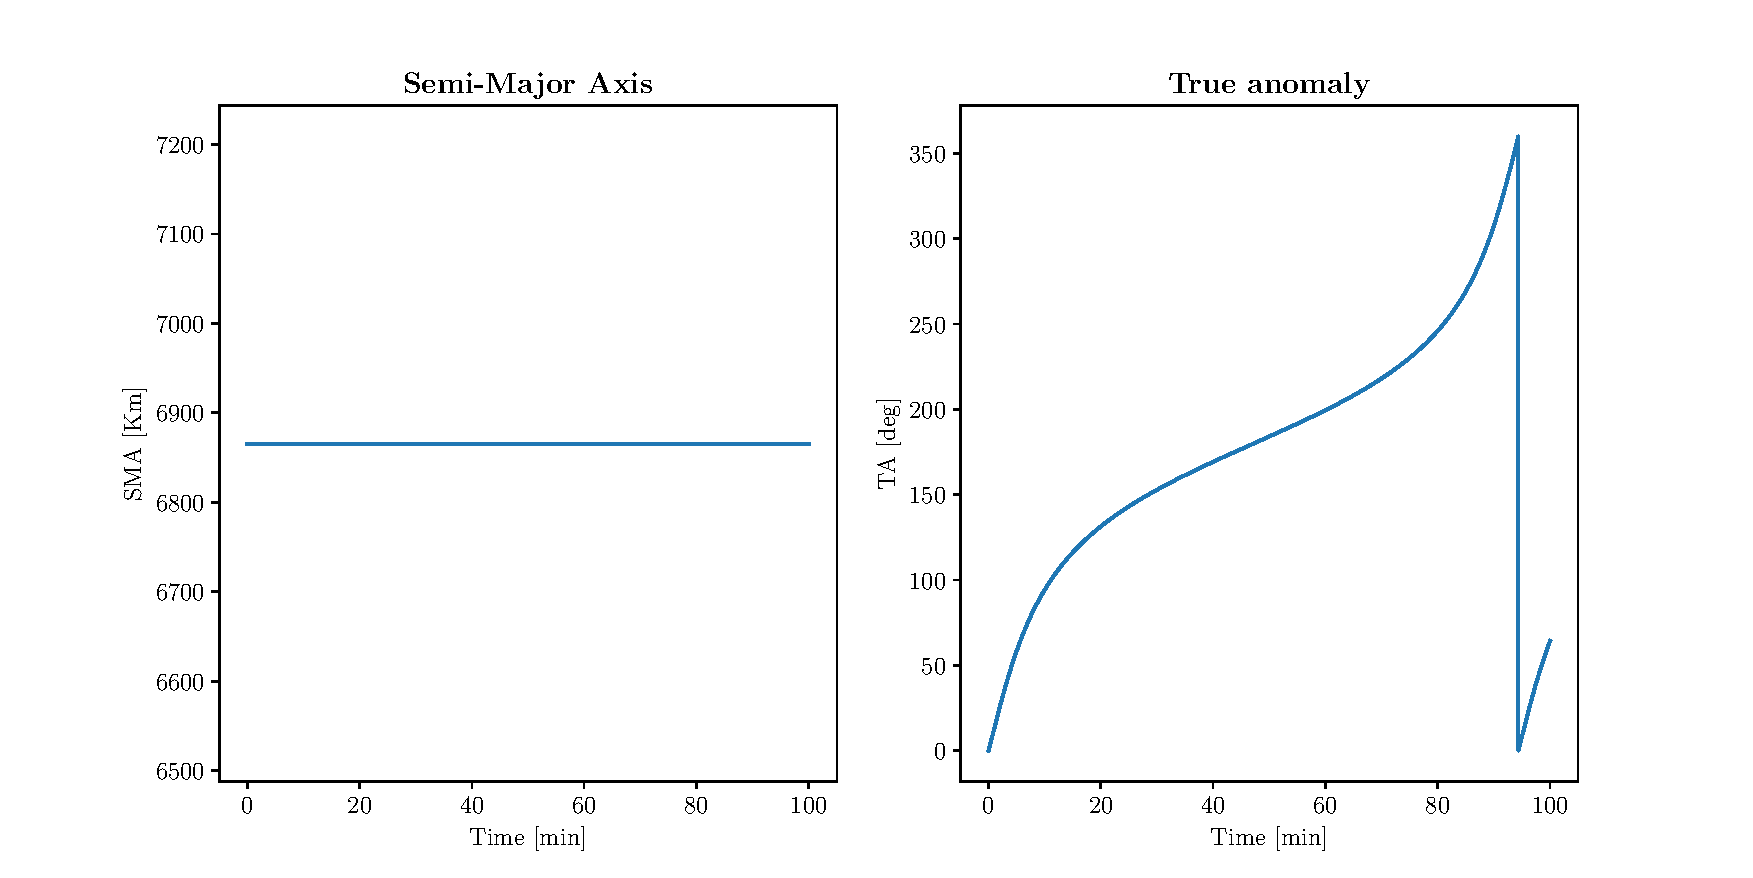
\includegraphics[scale=0.5]{img/keplerian_elements_high_ecc.pdf}
      \caption{SMA and true anomaly variation along around one LEO satellite orbit with eccentricity of 0.5}
      \label{kep_high_ecc_fig}
\end{figure}

All the case studies of this research consist of near-circular orbits.
Despite the fact that zero-eccentricity condition is not feasible, this comparison demonstrates that very low values of eccentricity would make the assumption of circular orbit highly acceptable.
Therefore, the Edelbaum-Kechichian formulas (paragraph \ref{station_keeping_par}) adopted for the station-keeping maneuvers are largely suitable for the problems addressed along the thesis.  


\subsection{Perturbed Motion}
The propagators developed by this work which take into account perturbing effects are based on the Cowell's technique of subsection \ref{orbit_prop_paragraph}.

Since Sun-synchronous orbits at low altitudes denote the main discussion point of this thesis, Earth's oblateness and atmospheric drag represent the perturbations of greatest interest. 
Despite this, propagations with SRP and 3rd-body forces have been examined as well for assessing long-term effects. 

The perturbing acceleration functions performed by this thesis come from the poliastro's library.


\subsubsection{Atmospheric Models}
The atmospheric drag exponential model provided by poliastro has been found to be too approximate compared to the results obtained by GMAT of equal examples.
For this reason, two more accurate atmospheric models have been implemented into the scripts designed along this work.
The first one consists of COESA76 model, while the second is the JB2008 one.
Their theoretical background has been already exposed in paragraph \ref{orbit_prop_paragraph}.
JB2008 is definitely the most accurate model


\subsubsection{Mean Orbital Elements Converter}


\subsubsection{Sun Synchronous Orbits Functions}


\subsection{Satellite Constellation Propagator}



\section{Differential Drag Controller} \label{differential_drag_control_par}
The differential drag algorithm represents the main effort of this thesis.
It consists of a method to perform the phasing through the differential drag of two or more satellites, of any shape and mass, after their deployment at the beginning of the mission.
The goal is to achieve an assigned orbital slot and same mean semi-major axis respectively on all spacecraft forming the constellation, resulting in zero relative velocity between them.
Since the algorithm designed by this thesis takes inspiration from the controller adopted by Planet (Foster et al. \cite{foster2015orbit}), a description of the latter is presented.

\subsection{Planet's Control Algorithm} \label{planet_algorithm_par}
The objective of Planet's algorithm is the same as that of the thesis.
The technique consists of labeling the satellite in the lowest orbit as the leading satellite.
Then, a two-component state composed by the mean Earth-centered angular distance to its desired slot $\theta_i$, and the angular velocity $\dot{\theta}_i$ relative to the leader, is computed for each trailing satellite.
The procedure to achieve the wanted pattern is reported below in the identical form presented by the company \cite{foster2015orbit}.

\begin{algorithm}[H]
      \caption{\textbf{Planet's Control}}
      \begin{algorithmic}[1]
            \Procedure{Create high-drag windows}{} 
                  \State remove any previously issued high-drag windows
                  \State compute $\theta_i$, $\dot{\theta}_i$ of each satellite \textit{i} relative to previous leader (mean, not osculating)
                  \State compute $\ddot{\theta}$ of a satellite in high-drag vs. low-drag mode
                  \State assign leader to be satellite with greatest $\dot{\theta}$ (i.e. lowest altitude)
                  \For{each satellite \textit{i} that is not the leader}
                        \State offset $\theta_i$, $\dot{\theta}_i$ to be relative to new leader: $\theta_i = \theta_i - \theta_{leader}, \dot{\theta}_i = \dot{\theta}_i - \dot{\theta}_{leader}$
                        \State get required high-drag duration to null relative speed with leader: $\Delta t_{i,hd} = - \frac{\dot{\theta}_i}{\ddot{\theta}}$
                        \State get angle travelled during desired high-drag window: $\theta_{i,hd} = \frac{1}{2} \ddot{\theta} \Delta t_{i,hd}^2$
                        \State get wait time to target desired slot: $\Delta t_{i,wait} = \frac{\theta_{i,hd} - \theta_i}{\dot{\theta}_i}$
                        \State create high-drag window for satellite \textit{i} starting at $t_{now} + \Delta t_{i,wait}$ for duration $\Delta t_{i,hd}$
                  \EndFor
            \EndProcedure
      \end{algorithmic}
\end{algorithm}

The strategy is to first obtain the high-drag time $\Delta t_{i,hd}$ (high-drag window) needed by the trailing satellite for matching the leader's semi-major axis, and then the amount of time $\Delta t_{i,wait}$ each spacecraft has to wait in the low-drag configuration before the high-drag maneuver is initiated.

Despite this method has successfully worked for the initial orbit phasing of a satellite constellation, it presents some limitations and ambiguities.
The durations $\Delta t_{i,wait}$ and $\Delta t_{i,hd}$ are predicted making assumptions related to the density of the atmosphere and the attitude of the vehicles.
This leads to unavoidable errors in accuracy.
In addition, it is not clear how the angular acceleration $\ddot{\theta}$ is estimated.
The angle $\theta_{i,hd}$ might also contain inaccuracies because is computed via Taylor approximation.
The accuracy of the algorithm is then strongly sensitive to the initial conditions of dispersion.
Too small differences between satellite orbits do not allow the control to function properly, as well as too big variations lead to inaccurate results.
Despite these negative observations, this algorithm has successfully worked for the initial phasing of a satellite constellation.
The Taylor approximation seems to be quite effective according to the on-orbit results shown in figure \ref{planet_orbit_results_fig} \cite{lee2017cubesat}.
The curves on the graph represent the relative angular distance between each satellite and the leader (which remains at zero degrees in the plot), and the blue lines are the high-drag windows.  
Indeed, Planet reruns its algorithm on a regular cycle to minimize the errors deriving from the forecast of the future state of the atmosphere.
As for the initial dispersion, it can be adjusted always through differential drag maneuvers, in order to achieve more proper initial conditions for the controller \cite{foster2015orbit}.
However, there is no clear information about the appropriate circumstances which make the algorithm work correctly.

\begin{figure}
      \centering
      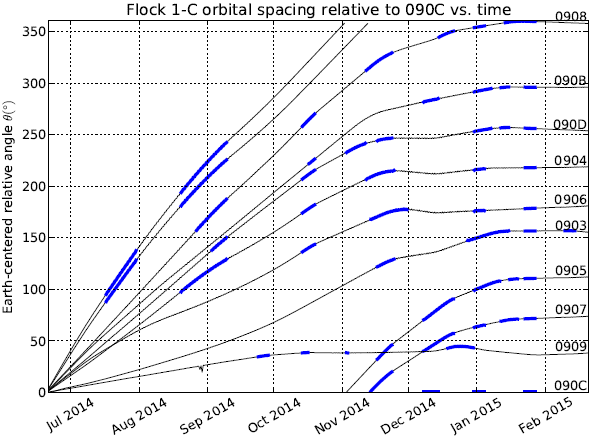
\includegraphics[scale=0.7]{img/planet_orbit_results.png}
      \caption{Actual Planet's fleet relative motion achieved by using differential drag. 
      Blue lines represent high-drag windows \cite{foster2015orbit}.}
      \label{planet_orbit_results_fig}
\end{figure}

Planet has applied this tool to groups of propulsion-less spacecraft.
Once the desired formation is achieved, the same differential drag control is used to maintain the requested relative angular distances between the vehicles.



\subsection{Thesis Controller}
This paragraph contains the work carried out to achieve the main goal of this thesis: the design of a differential drag controller for the initial orbit phasing of a group of spacecraft.
This is then combined with a low-thrust relative station-keeping.
Their coupling enables the orbital management of a LEO SSO constellation of low-thrust satellites throughout the mission lifetime. 
The drag control derives from an improvement of the Planet's algorithm.

First essential requirement is the use of the mean orbital elements.
All the space vehicles involved are supposed to have the same initial orbital elements except SMA and argument of latitude, and all the operations require the use of the mean orbital elements.

The algorithm establishes a reference vehicle, the \textit{leading satellite}, which is identified by the spacecraft travelling in the lowest orbit (greatest mean motion $n$).
The \textit{trailing satellites} have the task of reaching the desired relative placement with respect to the leader.
For each of them, the script computes the distance from the leader by the mean motion, the angular error $\theta_{err}$ from their position to the relative target, and the first attempt value of $t_{est}$.
Angular separations are calculated in terms of argument of latitude.
The latter parameter represents the interval of time in which the algorithm evaluates the variation of $n$.
$\dot{n}$ derives from the acceleration generated by the switch from low-drag to high-drag configuration.
This lead to the assessment of $t_{hd}$, the high-drag window.
After that, the algorithm evaluates the path travelled in high-drag configuration $\theta_{hd}$ and finally the wait time $t_{wait}.$ 
At this point, the estimation of $t_{hd}$ and $t_{wait}$ is repeated with a new $t_{est}$ provided by a function which depends on the altitudes of the satellites and the time intervals computed before.
The procedure is rerun for a sufficient number of iterations.
The procedure is shown below.

\begin{algorithm}[H]
      \caption{\textbf{Differential Drag Control}}
      \begin{algorithmic}[1]
            \Procedure{Perform phasing through differential drag}{} 

                  \State establish the leading satellite (greatest mean motion)

                  \For{each trailing satellite of the constellation}

                  \State compute difference in mean motion with respect to the leader $\Delta n$
                  \State compute angle to reach the desired slot relative to the leader $\theta_{err}$ 
                  \State assign first attempt value to $t_{est}$ from $\theta_{err}$  
                                        
                        \For{assigned number of iterations}
                              
                              \State get mean motion variation $\dot{n}$ from low to high drag mode over $t_{est}$
                              \State get high drag time window $t_{hd} = \frac{\Delta n}{\dot{n}}$
                              \State get angle travelled during high drag window $\theta_{hd} = \frac{1}{2}\dot{n}t_{hd}^2$
                              \State get waiting time window $t_{wait} = \frac{\theta_{err} - \theta_{hd}}{\Delta n}$
                              \State get new estimation time $t_{est} = f(t_{wait}, t_{hd}, h_{lead}, h_{trail})$ 
                        \EndFor
                  \EndFor
            \EndProcedure
      \end{algorithmic}
\end{algorithm}

The strong point of the proposed method lies in the last line.
The estimation time is a critical factor in terms of accuracy for the final result.
It is estimated thanks to an empirical equation formulated within this thesis work.
This function enables a significant better prediction of the two time windows, making unnecessary the rerun of the algorithm in several cases.
Despite this, regular repetition of the calculations remains a good and sometimes necessary action as for the Planet's strategy.
$t_{est}$ is evaluated for an assigned number of iterations, but the experience shows that just twice in enough.
The statements above as will be proven in chapter \ref{results_chapter}.
Similarly to Planet's algorithm, this method is sensitive to the initial dispersion after the deployment.
However, this is issue is easily addressed implementing preliminary high-drag or wait windows.
The only determining factors of this problem are the initial difference in semi-major axis and the altitude from which the launcher deploys the satellites.
The first condition is managed with proper high-drag maneuvers.
On the other hand, when the deployment altitude it is too high, differential drag is unavoidably too low.
Therefore, a preparatory wait time window might be required for the entire fleet of spacecraft, eventually applying high-drag mode to them in order to speed up the process.



\section{Station-Keeping Simulator} \label{sk_simulator_par}
This tool is an absolute station-keeping simulator.
It is able to simulate actions of IAM and DMU performed by low-thrust propelled satellites.
The method combines an orbit propagator and an algorithm that keep the spacecraft within a defined range of altitudes and inclinations.
The required input parameters include the thrust force of the propulsion system as well as the edge values of the orbital elements that define the station-keeping box (paragraph \ref{station_keeping_par}).
The simulator works with the perturbations, therefore it is indispensable to deal with the mean orbital elements to carry out the maintenance.

The logic behind the method is shown below.
\begin{algorithm}[H]
      \caption{\textbf{Station-Keeping Simulation}}
      \begin{algorithmic}[1]
            \Procedure{Simulate the absolute station-keeping of a spacecraft}{} 
                  \For{each time step in the time frame}
                        \State propagate the satellite's orbit
                        \If{current mean SMA < lower SMA}
                            \While{current mean SMA < upper SMA}
                                \State activate thruster
                            \EndWhile
                        \EndIf           
                        \If{current mean inclination < lower inclination value}
                            \While{current mean inclination < upper inclination value}
                                \State activate thruster
                            \EndWhile
                    \EndIf
                  \EndFor
            \EndProcedure
      \end{algorithmic}
\end{algorithm}

The algorithm uses the Edelbaum-Kechichian theory reported in subsection \ref{station_keeping_par}.
However, a careful observer would notice that actually the script takes advantage of this theory only to compute the yaw angle (equation \ref{yaw_angle_equation}) in case of out-of-plane maneuver (change in inclination).
Indeed, the burning time estimated by the equations is never taken into account.
The update of the satellite's position at each time step allows a better accuracy which otherwise would be affected by the uncertainties generated by the unpredictable factors of the perturbing effects over a long time interval.

Nevertheless, the equations of the Kechichian's method are used to provide the $\Delta V$ required by the station-keeping, which is a fundamental parameter for the mission designer.



\section{Revisit Time Collector} \label{revisit_time_collector_par}
The revisit time collector (RTC) tool intends to compute the amount of passages of a satellite above a specific position on Earth.
It collects the \textit{access times} of the spacecraft when its target on the ground is within the area delimited by the swath width of the satellite's on-board camera. 
It can work with a single space vehicle or with a constellation. 
In the latter case, the script provides all the access times taking into account every single satellite of the pattern. 

In addition to the input parameters required by the selected propagator (paragraph \ref{orbit_propagators_par}), the RTC needs the target coordinates in latitude and longitude, as well as the swath width of the electro-optical sensor.
The algorithm computes the distance between the sub-satellite point on the ground and the target at each time step.
This calculation is performed considering some meaningful aspects.

The goal of the RTC clearly requires the estimation of the satellite's position in an ECEF reference frame.
If its motion was evaluated with respect to an ECI system, the ground track of the orbit would be always the same after each orbital period.
ECEF coordinates shall be then converted into the geodetic latitude-longitude location of the spacecraft's subpoint in order to proceed with the distance calculation.

The computation of the distance between two points on the Earth surface shall take into account the sphericity of the planet.
To accomplish this condition, the algorithm computes the so-called geodesic distance, which can be defined as the shortest path between two points on the surface of an ellipsoidal model of the Earth. 
As regards the geodetics, the script takes advantage of the method proposed by Karney \cite{karney2013algorithms}.

Summarizing, the algorithm extracts the sub-point latitude and longitude from the ECEF state vector of the satellite and, after that, calculates the geodesic distance with respect to the ground target.
This path is then compared with half the value of the potential swath width (PSW) at each time step of the propagation.
If the distance is smaller than PSW then the script saves the epoch related to that time step.

\begin{algorithm}
      \caption{\textbf{Revisit Time Collection}}
      \begin{algorithmic}[1]
            \Procedure{Collect revisit time epochs over a specific target}{} 
                  \State propagate the satellite's orbit for the desired time frame
                  \For{each time step in the time frame}
                        \State convert satellite state vector from ECI to ECEF
                        \State extract geodetic latitude and longitude
                        \State compute the geodesic distance between target and sub-satellite point
                        \If{distance between the two points < $\frac{PSW}{2}$}
                              \State collect the epoch of the current time step
                        \EndIf
                  \EndFor
            \EndProcedure
      \end{algorithmic}
\end{algorithm}

It is important to underline that the actual sensor input value to be implemented in the RTC should be related to the concept of \textit{potential swath coverage}.
It identifies the potential path reachable by a pointable space system.
If the satellite can not work off-nadir then the input parameter will be simply equal to half the SW due to the fact that the subpoint always lies in the middle of the observed area.
Therefore, according to the figure \ref{potential_sw_fig}, a proper use of the algorithm should get half the potential swath width (PSW) as input value.
\begin{figure}[H]
      \centering
      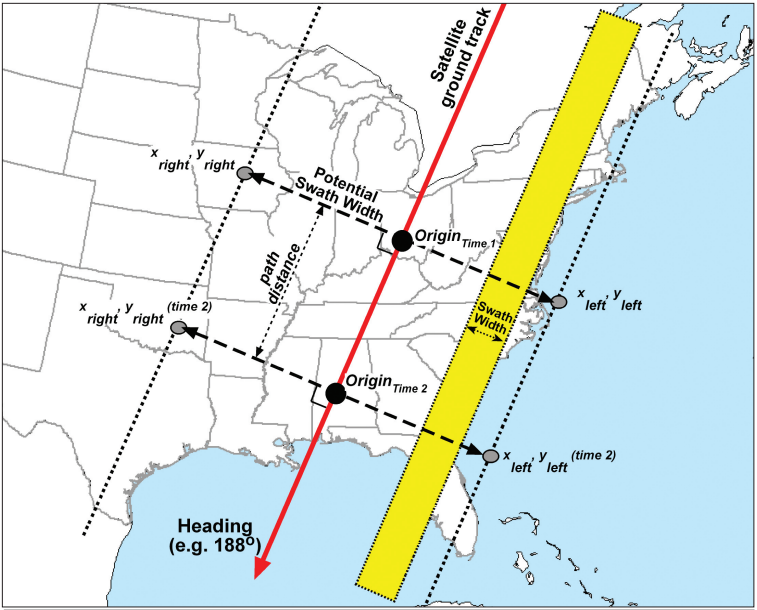
\includegraphics[scale=0.6]{img/potential_sw.png}
      \caption{Projection of satellite ground track and potential swath width with respect to its swath width at two time steps \cite{hodgson2008modeling}.}
      \label{potential_sw_fig}
\end{figure}